\section{ Evaluation and Validation}\label{sec:acc_eval}
To validate our model, several metrics are taken to measure the performance of
our model.
Although random forests are less likely to overfit, it can still occur, and is
nonetheless important to detect.

Most metrics, natively suited to binary classifiers, are easily adapted for use
in multi-class tasks.
It is equally important to correctly sample the data as to avoid bias.
This section discusses first the framework around which the performance of our
model is measured, the metrics used, and finally an analysis of the results.

Section~\ref{sec:tuning} analyses the performance of the classifier with varying
parameters, in order to find their optimal values.

\subsection{Validation Strategy and Sample Space}
In effort to reduce sensitivity to chance selection of random samples, all
measurements are performed using a multi-run stratified 10-fold cross validation.
This gives us a 90/10 train/test data split, and is repeated with a new random
sample shuffling 10 times.
Stratification ensures that there exists an equal class balance in the testing
and training splits, so that all classes are represented equally.

This is especially important given the small number of representative samples
for each class.
Advanced methods exist in order to futher improve our results, such as
bootstrapping, but this has not been pursued.
Note that random forests use bootstrap sampling, where a portion of the data is
not used for training.
This does produce a measurable result similar in effect to cross-validation,
called the OOB error, discussed in Section~\ref{sec:metrics}.

For each fold, only features from the selected training samples are
used for training and validation.

A total of 3 batches have been computed and merged, giving 12 species in total.
Selection was performed using the mechanisms outlined in
Section~\ref{sec:sample_select}.
Table~\ref{tbl:used_data} shows the selection of species including spectrogram
and template counts per species.

\begin{table}[!htb]
  \caption{Selected species with spectrogram and template counts}
  \label{tbl:used_data}
  \centering
  \begin{tabular}{l r r}
    Species Label & Spectrograms & Templates \\ \hline
    Common Blackbird           & 20 & 6132\\
    Great Reed Warbler         & 20 & 5111\\
    Common Rosefinch           & 20 & 3191\\
    Common Cuckoo              & 20 & 2909\\
    Common Chiffchaff          & 20 & 2886\\
    European Greenfinch        & 20 & 2759\\
    Pale-breasted Spinetail    & 20 & 2501\\
    Ortolan Bunting            & 20 & 2362\\
    Common Reed Bunting        & 20 & 2233\\
    Chestnut-breasted Wren     & 20 & 2203\\
    Corn Bunting               & 20 & 2082\\
    Rufous-browed Peppershrike & 20 & 1404\\ \hline
    \multicolumn{1}{r}{Total} & 240 & 35773
  \end{tabular}
\end{table}

\subsection{Evaluation Metrics}\label{sec:metrics}
Each of the five following evaluation metrics are computed in a fold.
They are then stored and averaged at the end of the cross validation.

\begin{itemize}
  \item \textbf{Accuracy}
    Is the ability of the classifier to correctly label samples.
    \begin{equation}
      \frac{TP+TN}{P+N}
    \end{equation}

  \item \textbf{Precision},
    Sometimes referred to as the positive predictive value, is the ability of the
    classifier to label all predicted values correctly.
    \begin{equation}
      \frac{TP}{TP+FP}
    \end{equation}

  \item \textbf{Recall},
    Sometimes referred to as sensitivity, is the ability of the classifier to
    label all positive samples correctly.
    \begin{equation}
      \frac{TP}{P}
    \end{equation}

  \item \textbf{F-beta score}
    Is the weighted harmonic mean of the precision and recall, where
    higher values indicate better performance.
    This makes it simpler to compare the performance of different parameter sets.
    \begin{equation}
      \frac{(1+\beta^2)TP}{(1+\beta^2)TP+\beta^2FN+FP}
    \end{equation}

    We consider precision and recall as equally important, in which case the
    beta value is set to 1:
    \begin{equation}
      \frac{2TP}{2TP+FN+FP}
    \end{equation}

  \item \textbf{OOB error rate}
    Is the out-of-bag (OOB) samples are those which were not selected during the
    construction of a specific tree.
    Given the most common label from classifying a sample with its respective tree,
    the porportion of incorrect classifications is averaged over all OOB samples
    is taken as the OOB error rate on the training data.

\end{itemize}

The Scikit Learn |precision_recall_fscore_support| function was used to compute
these metrics.

Because this is a multi-class classification task, each metric is computed
on a per-label basis.
The average is then computed using "macro" averaging, in which the mean of each
score is computed with equal weighting for all labels.
This is appropriate considering we use stratified k-fold, and each
species is considered equally important to all the others.

\subsubsection{Results}
Results are promising, good performance has been achieved using the initial
parameters, with observed improvements after tuning as is shown in
Table~\ref{tbl:acc_before_after}.

\textbf{update w/ new defaults}
\textbf{wait for gs results... }
\begin{table}[!htb]
  \centering
  \caption{Comparison of accuracies using default and tuned parameters}
  \label{tbl:acc_before_after}
  \begin{threeparttable}
    \begin{tabular}{l r r}
      & \multicolumn{2}{c}{Metric Scores} \\
      Metric    & Default Params. & Tuned Params. \\ \hline
      Accuracy  & 79.5 (7.3) & 0 \\
      F1 Score  & 77.9 (8.1) & 0 \\
      Recall    & 79.5 (7.4) & 0 \\
      Precision & 82.3 (8.5) & 0 \\
      OOB Error & -- & --
    \end{tabular}
    \begin{tablenotes}
      \footnotesize
      \item[*] Values are shown as percentages.
      \item[*] Standard deviations are shown in parentheses.
    \end{tablenotes}
  \end{threeparttable}
\end{table}

\subsection{Confusion Matrix}
A confusion matrix plots the rate at which each label is predicted as any other
label, where the rows represent the true label, and columns represent the
classifier's predictions.

We construct a confusion matrix to evaluate the performance of the classifier
and the features used to discriminate between species.
In this case the matrix allows us to visualise the performance distribution per
class, and give
some insight into how the classifier is responding to the selected features.

Figure~\ref{fig:cnf12} shows the resulting confusion matrix from classifying the
selected data, averaged over the 10-run 10-fold cross validation.
Row-wise normalisation was performed.

\begin{figure}[!htb]
  \centering
  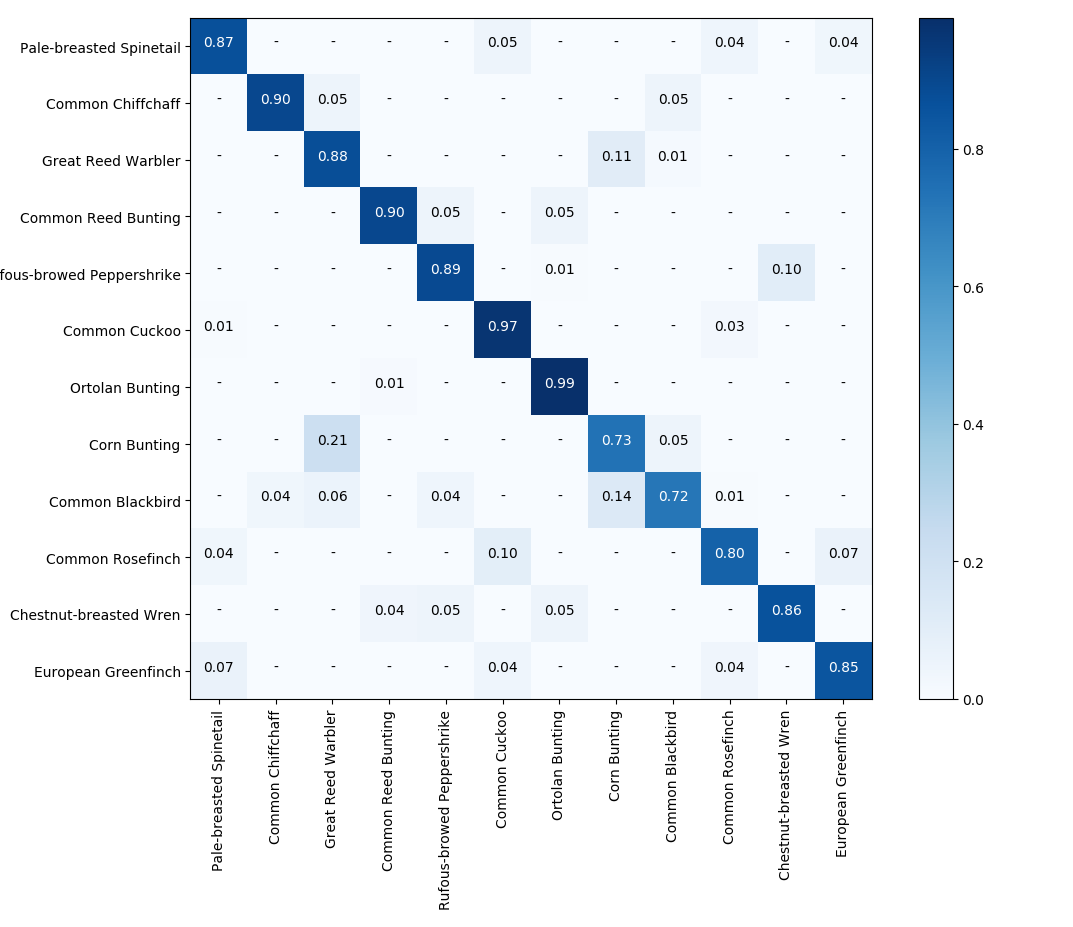
\includegraphics[width=1.0\textwidth]{cnf_matrix_12}
  \caption{Row-Normalized Confusion Matrix}\label{fig:cnf12}
\end{figure}

The confusion matrix shows good classification performance for most species.\\

We can see from the results that the Common Blackbird is the worst performing
classification with a 40\% false negative rate.
It is often mistaken for a Great Reed Warbler, but not the other way around,
which may indicate weakness in the Common Blackbird's templates.

... more speculation

Aside from computing the metrics shown in Section~\ref{sec:metrics}, a confusion
matrix can only offer a speculative insight into template performance.
Nonetheless, it offers a starting point into further template analysis as
discussed in Section~\ref{sec:template_analysis}.
